\documentclass[11pt,xcolor=svgnames]{beamer}
\usepackage{dsfont,natbib,setspace,changepage,multirow}
\mode<presentation>

% fonts

% replaces beamer foot with simple page number
\setbeamertemplate{navigation symbols}{}
\setbeamercolor{frametitle}{fg=black}
\setbeamerfont{frametitle}{series=\bfseries}
\setbeamerfont{frametitle}{size=\normalsize}

\newcommand{\theme}{\color{Maroon}}

\setbeamertemplate{footline}{
   \raisebox{5pt}{\makebox[\paperwidth]{\hfill\makebox[20pt]{\color{gray}\scriptsize\insertframenumber}}}}

\graphicspath{{../graphs/}}

%\setbeamercolor{whitebox}{bg=gray!10}

% colors
\newcommand{\bk}{\color{black}}
\newcommand{\rd}{\color{red}}
\newcommand{\fg}{\color{ForestGreen}}
\newcommand{\bl}{\color{blue}}
\newcommand{\gr}{\color{black!60}}
\newcommand{\sg}{\color{DarkSlateGray}}
\newcommand{\br}{\color{SaddleBrown}}
\newcommand{\nv}{\color{Navy}}
\setbeamercolor{itemize item}{fg=gray}

% common math markups
\newcommand{\bs}[1]{\boldsymbol{#1}}
\newcommand{\mc}[1]{\mathcal{#1}}
\newcommand{\mr}[1]{\mathrm{#1}}
\newcommand{\bm}[1]{\mathbf{#1}}
\newcommand{\ds}[1]{\mathds{#1}}
\newcommand{\indep}{\perp\!\!\!\perp}

% spacing and style shorthand
\setstretch{1.1}

% shorthand
\newcommand{\sk}{\vspace{.5cm}}
\newcommand{\R}[1]{{\tt \nv #1}}
\newcommand{\til}{{\footnotesize$\bs{\stackrel{\sim}{}}$}}
\DeclareSymbolFont{extraup}{U}{zavm}{m}{n}
\DeclareMathSymbol{\vardiamond}{\mathalpha}{extraup}{87}

\begin{document}

\setcounter{page}{0}
{\setbeamercolor{background canvas}{bg=MidnightBlue}
\begin{frame}[plain]



\color{white} \sf {\Huge  A Primer on Machine Learning}

\vskip 1cm
ABFER 2017 -- Singapore\\
Masterclass part II\\
Matt Taddy

\end{frame}}

\begin{frame}

\sf \LARGE
\begin{center}
ML is fast semiparametric prediction with \\{\gr Bayesian} heuristics to avoid overfit
\end{center}
\end{frame}

\begin{frame}
{What is ML?}

\vskip .5cm
ML combines flexible semiparametric models with fast estimation algorithms and tools that ensure out-of-sample validity.

\vskip .5cm
{\theme Supervised} ML is trained to minimize loss on a small set of outcomes `y'.  {\nv Unsupervised} ML loss is defined over all variables.

\vskip .5cm
ML discovers patterns in the DGP.\\
It's backwards looking: predicts a future that behaves like the past.\\

\end{frame}

\begin{frame}
{The plan}

Out-of-Sample vs In-Sample performance

\vskip .5cm 
Regularization paths, the lasso, and penalty selection

\vskip .5cm 
Trees, forests, and regularization via the bootstrap

\end{frame}


\begin{frame}
{{\nv Example:} Semiconductor Manufacturing Processes}

\begin{columns}[c]

\column{1.75in}

\vskip .25cm

\includegraphics[width=2in]{schalfhigh}
\column{2in}\small
\begin{center}


Very complicated operation\\
{\sg Little margin for error.}


\vskip .25cm
Hundreds of diagnostics\\
{\sg Useful or debilitating?}

\vskip .25cm
We want to focus reporting and
better predict failures.

\end{center}

\end{columns}

\sk
$\bm{x}$ is 200 input signals, $y$ has 100/1500 failures.

\vskip .25cm
Logistic regression for failure of chip $i$ is

\vspace{-.25cm}
\[p_i = \mr{p}({\tt fail}_i|\bm{x}_i) = e^{\alpha+\bm{x}_i\bs{\beta}}/(1+ e^{\alpha+\bm{x}_i\bs{\beta}})
\]


% The $x_{ij}$ inputs here are actually orthogonal: they are the first 200 Principal Component directions from an even bigger set.

\vspace{-.25cm}

\end{frame}

\begin{frame}
{Semiconductor FDR Control}

The full model has $R^2 = 0.56$ {\gr (based on {\it binomial} deviance)}.

The p-values for these 200 coefficients:


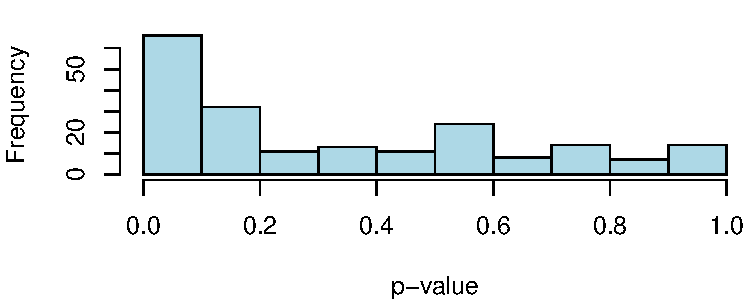
\includegraphics[width=4.1in]{../graphs/SCpvals}

\vskip .25cm

{\gr Some are clustered at zero, the rest sprawl out to one.}\\

FDR of $q=0.1$ yields  $\alpha=0.0122$ p-value rejection cut-off. \\Implies 25 `significant', of which approx 22-23 are true signals.

\end{frame}


\begin{frame}
{semiconductors}

A {\it cut} model, using only these 25  signals,
has $R_{cut}^2 = 0.18$.  \\
This is much smaller than the full model's $R_{full}^2=0.56$.

\sk
In-Sample (IS) $R^2$ {\it always} increases with more covariates.
\\ {\gr This is exactly what MLE $\bs{\hat\beta}$ is fit to maximize.}
\\ {\theme But how well does each model predict {\it new} data?}

\sk
{ An out-of-sample (OOS) experiment}
\begin{itemize}
\item split the data into 10 random subsets {(`folds')}.
\item Do 10x: fit model $\bs{\hat\beta}$ using only 9/10 of data, 
\\ ~~~~~~~~~~~and record $R^2$ on the left-out subset. 
\end{itemize}
These OOS $R^2$ give us a sense of how well each \\model can predict
data that it has not already seen.
\end{frame}

\begin{frame}
{OOS experiment for semiconductor failure}

We gain predictive accuracy by {\it dropping} variables.

\begin{center}\vspace{-.2cm}
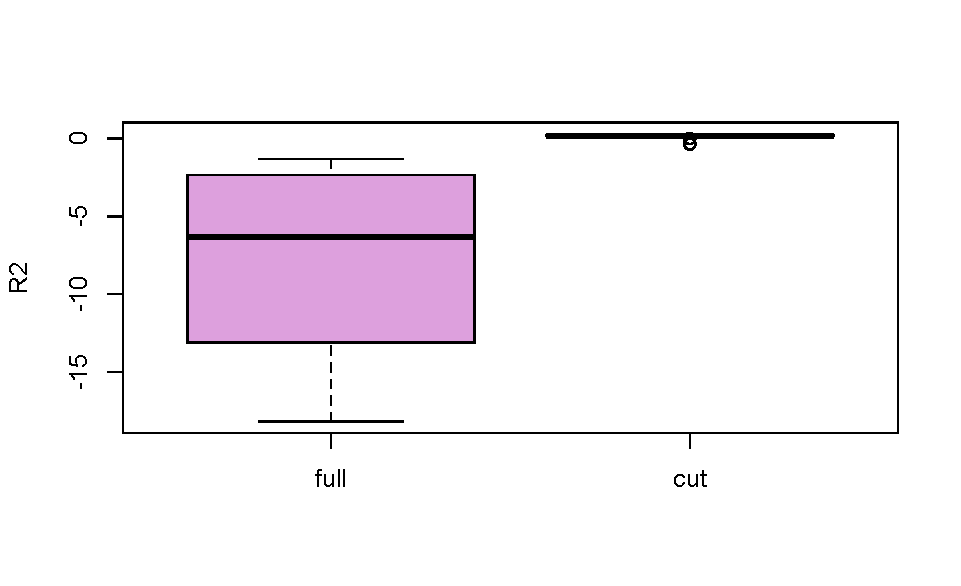
\includegraphics[width=4in]{SCr2}
\end{center}

Cut model has mean OOS R2 of 0.09, about 1/2 in-sample R2.

\vskip .2cm
The full model is terrible.  It is overfit and worse than $\bar y$.\\ 
{\nv Negative R2 are more common than you might expect.}

\vspace{-.2cm}
\end{frame}

\begin{frame}
{OOS experimentation}

{\nv All that matters is Out-of-Sample $R^2$.}  \\{\theme We don't care about In Sample $R^2$.}

\sk
Using OOS experiments to  choose the best model is called {\it cross validation}.  It will be a big part of our big data lives.

\sk
Selection of `the best' model is at the core of all big data.

\vskip .1cm
But before getting to selection, we first need strategies to \\ build good sets of candidate models to choose amongst.

\end{frame}


\begin{frame}
{Naive forward stepwise regression}

\vskip .25cm
The {\tt \nv step()} function in R executes a common routine:

\vskip .05cm
\begin{itemize}
\item Fit all univariate models.  
Choose that with highest (IS) $R^2$ \\
 and put that variable -- say $x_{(1)}$ -- in your model.
\item Fit all bivariate models including $x_{(1)}$ 
($y \sim \beta_{(1)}x_{(1)} + \beta_jx_j$), 
and add $x_j$ from one with highest $R^2$ to your model.
\item Repeat:  max $R^2$ by adding one variable to your  model.
\end{itemize}

\vskip .05cm
You stop when some model selection rule (AIC) is lower for the
current model than for any of the models that add one variable.

\end{frame}

\begin{frame}
{The problem with Subset Selection}


{\tt \nv step()} is very slow {\gr (e.g., 90 sec for tiny semiconductors)}

\vskip .5cm
This is true in general with {\theme subset selection} (SS): 

\vskip .1cm
Enumerate candidate models by applying maximum likelihood estimation for subsets of coefficients, with the rest set to zero.

\vskip .5cm
SS is slow because adding one variable to a regression can change fit dramatically: {\it each model must be fit from scratch}.

\vskip .5cm
A related subtle (but massively important) issue is {\theme stability}.

\vskip .1cm MLEs have high {\it sampling variability}: they change a lot from one dataset to another.  So which MLE model is `best' changes a lot.

\vskip .1cm $\Rightarrow$ you won't know where to stop stepping.

\end{frame}



\begin{frame}
{Regularization}

The key to contemporary statistics is
{\nv regularization:} \\~~~~~~~~~~~~~~~depart from optimality to stabilize a system.

{\gr Common in engineering: I wouldn't drive on an optimal bridge.}

\vskip .5cm
We minimize deviance \onslide<2->{{\nv plus a cost on the size of
coefficients.}} {\large\begin{equation*}
\mr{min} 
-\frac{2}{n}\log \text{LHD}(\bs{\beta}) 
\onslide<2->{{\nv + \lambda\sum_k |\beta_k|}}
\end{equation*}}

\vskip -.25cm
\onslide<2>{This particular cost gives the `lasso': the new least squares.}

\end{frame}


\begin{frame}
{Decision theory: \theme Cost in Estimation}


Decision theory is based on the idea that choices have costs.\\
Estimation and hypothesis testing: what are the costs?


\sk 
{\nv Estimation:}

\vskip .1cm
Deviance is the cost of distance between data and the model.\\
{\gr Recall: $\sum_i (y_i-\hat{y}_i)^2$ or 
$-\sum_i y_i\log(\hat{p}_i) - (1-y_i )\log(1-\hat{p}_i)$.}

\vskip .25cm
{\nv Testing:}

\vskip .1cm
Since $\hat{\beta}_j = 0$ is  {\it safe},  it should cost us to
decide otherwise.

\sk 
$\Rightarrow$ The cost of $\hat{\beta}$ is deviance plus
a penalty  away from zero.



\end{frame}


\begin{frame}
{{\gr [Sparse]}  Regularized Regression}


{\nv\large\[
\mr{min} \left\{ -\frac{2}{n}\log\text{LHD}(\bs{\beta}) + \lambda \sum_j c(\beta_j)\right\}
\]}

$\lambda >0$ is the penalty weight, $c$ is a cost (penalty) function.

$c(\beta)$ will be lowest at $\beta=0$ and we pay more for $|\beta| > 0$.

\vskip .1cm
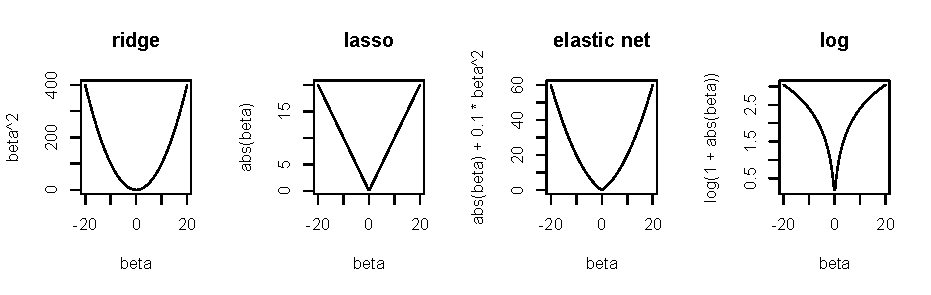
\includegraphics[width=4.25in]{penalties}

Options: ridge $\beta^2$, lasso $|\beta|$, elastic net $\alpha\beta^2 + |\beta|$,  $\log(1 + |\beta|)$.


\end{frame}


\begin{frame}
{Penalization can yield {\theme automatic variable selection}}

The minimum of a smooth + pointy function can be at the point.

\vskip -.25cm
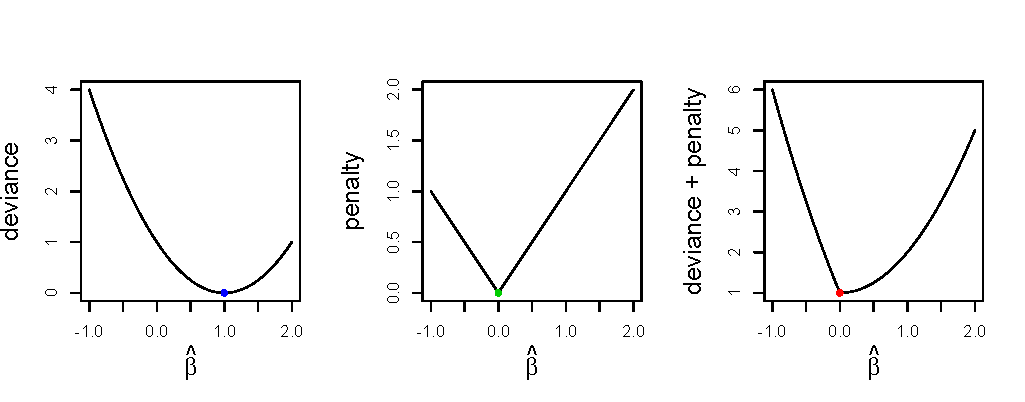
\includegraphics[width=4.25in]{penlasso}

\vskip .5cm
Anything with an absolute value (e.g., lasso) will do this.  

\vskip .1cm 
{\gr There are MANY penalty options and far too much theory.}

\vskip .1cm 
Think of lasso as a baseline, and others as variations on it.

\end{frame}

\begin{frame}
{Lasso Regularization Paths}


The lasso fits $\bs{\hat\beta}$ to minimize $-\frac{2}{n}\log\text{LHD}(\bs{\beta}) + \lambda \sum_j |\beta_j|$.

\vskip .1cm
We'll do this for a {\it sequence} of penalties $\lambda_1 > \lambda_2 ... > \lambda_T$.

\vskip .1cm
{\gr Then we can apply model selection tools to choose best $\hat \lambda$.}

\sk
{\nv Path estimation:}

\vskip .1cm
~~~ Start with big $\lambda_1$ so big that $\bs{\hat \beta}=\bm{0}$.

\vskip .1cm
~~~ For $t=2\ldots T$: update $\bs{\hat \beta}$ to be optimal under $\lambda_t < \lambda_{t-1}$.

\sk


Since estimated $\bs{\hat\beta}$ changes smoothly along this path:
\begin{itemize}
\item It's fast!  Each update is easy.
\item It's stable: optimal $\lambda_t$ may change a bit from sample to sample, but that won't affect the model much.
\end{itemize}
{\gr It's a better version of forward stepwise selection.}

\end{frame}


\begin{frame}
{Path plots}

\vskip .25cm
The whole enterprise is easiest to understand visually.

\vskip -.25cm
\begin{center}
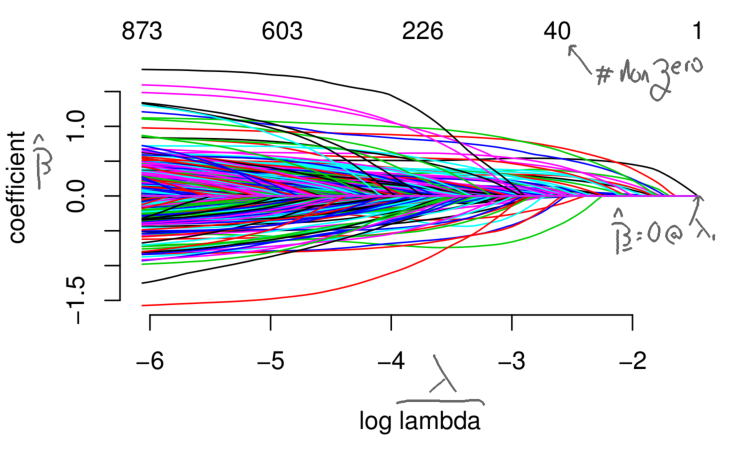
\includegraphics[width=.95\textwidth]{comscore_markeduppaths}
\end{center}

\vskip -.25cm
The algorithm moves {\it right to left}.  \\The $y$-axis is $\bs{\hat\beta}$ (each line a different $\hat\beta_j$) as a function of $\lambda_t$.
\end{frame}



\begin{frame}
{{\nv Example: } Comscore web browser data}

The previous plot is  household log-online-spend regressed onto $\%$ of time spent on various websites (each $\beta_j$  a different site).

\vskip .25cm
Comscore 
 (available via WRDS) records info on browsing\\ and purchasing behavior for annual panels of households.

\vskip .25cm

I've extracted 2006 data for the 1000 most heavily trafficked websites and for 10,000 households that spent at least 1\$.  


\vskip .25cm
Why do we care?  {\theme Predict consumption from browser history.}

\vskip .1cm
{
e.g., to control for base-level spending, say, in estimating advertising effectiveness.  
You'll see browser history of users when they land, but likely not what they have bought.  }


\end{frame}

\begin{frame}
{Lasso Software}


There are many packages for fitting lasso regressions in R.

\vskip .25cm
{\tt \nv glmnet} is most common.  {\tt \nv gamlr} is my contribution.

These two are very similar, and they share syntax.

\vskip .25cm
Big difference is what they do beyond a simple lasso:.

~~~{\tt\nv glmnet} does an `elastic net':  $c(\beta) = |\beta| + \nu \beta^2$.

~~~{\tt\nv gamlr} does  a `gamma lasso': $c(\beta) \approx \log(\nu + |\beta|)$.

\vskip .25cm  
Since we stick mostly to lasso, they're nearly equivalent for us.  {\tt \nv gamlr} just makes it easier to apply some model selection rules.

\sk
Both use the {\tt \nv Matrix} library representation for {\theme sparse matrices}.
\end{frame}


\begin{frame}[fragile]
{Running a lasso}

{Once you have your {\tt x} and {\tt y}, running a lasso is easy.}

\vspace{-.75cm}
\begin{semiverbatim}\small \nv
spender <- gamlr(xweb, log(yspend))
plot(spender) {\gr # nice path plot}
spender\$beta[c("mtv.com","zappos.com"),] 
\end{semiverbatim}

\vskip .25cm And you can do logistic lasso regression too

\vspace{-.75cm}
\begin{semiverbatim}\small \nv
gamlr(x=SC[,-1], y=SC\$FAIL, {\theme family="binomial"})
\end{semiverbatim}
\vskip -.25cm
{You should make sure that {\tt y} is numeric 0/1 here, not a factor.}

\vskip .5cm
See {\tt ?gamlr} for details and help.

\end{frame}


\begin{frame}
{Size Matters}

Penalization means that scale matters. {\gr e.g.,  $x\beta$ has the same effect as $(2x)\beta/2$, but $|\beta|$ is twice as much penalty as $|\beta/2|$.}

\sk
You can
multiply $\beta_j$ by sd($x_j$) in the cost function to standardize. 

\vskip .2cm
~~That is, minimize $-\frac{2}{n}\log\text{LHD}(\bs{\beta}) + \lambda \sum_j \mr{sd}(x_j)|\beta_j|$.

\vskip .2cm
~~$\Rightarrow \beta_j$'s penalty is calculated per effect of 1SD change in $x_j$.


\sk
{\tt gamlr} and {\tt glmnet} both have {\tt standardize=TRUE} by default.

{\theme You {\it only} use {\tt standardize=FALSE} if you have good reason. }


\end{frame}


\begin{frame}
{Regularization and Selection}



{The  lasso minimizes $-\frac{2}{n}\log\text{LHD}(\bs{\beta}) + \lambda \sum_j |\beta_j|$.}

\vskip .1cm
This `sparse regularization' auto-selects the variables.  

\vskip .1cm
{Sound too good to be true?  You need to choose $\lambda$.}

\sk
Think of $\lambda>0$ as a signal-to-noise filter: {\it like squelch on a radio.}



\sk We'll  use {\theme cross validation} or {\nv information criteria} to choose.


\sk
Path algorithms are key to the whole framework:

\vskip .1cm
$\star$ They let us quickly enumerate a set of candidate models.

$\star$ This set is stable, so selected `best' is probably pretty good.

\end{frame}



\begin{frame}
{{\nv Model Selection:} it is all about prediction.}

A recipe for model selection.
\begin{enumerate}\bk
\item Find a manageable set of candidate models \\{(i.e., such that fitting all models is fast).}
\item Choose amongst these candidates the one with\\ best
predictive performance {\it on unseen data}.
\end{enumerate}

\sk
{\nv 1.} is what the lasso paths provide.

\vskip .1cm
{\nv 2.} Seems impossible!  But it's not $\ldots$

\sk 
First, define {\nv predictive performance} via `deviance'. 

\vskip .1cm
Then, we need to {\it estimate} deviance for a fitted model applied to {\it new independent observations} from the true data distribution.

\end{frame}


\begin{frame}
{Out-of-sample prediction experiments}

\vskip .25cm
We already saw an OOS experiment with the semiconductors.
Implicitly, we were estimating predictive deviance (via $R^2$).

\vskip .25cm
The procedure of using such experiments to do model selection is
called {\theme Cross Validation} (CV).  It follows a basic algorithm:

\vskip .25cm

For $k = 1\ldots K$,
\begin{itemize}
\item Use a subset of $n_k < n$ observations to `train' the model.
\item Record the error rate for predictions from \\this fitted model on the left-out observations.
\end{itemize}

\vskip .25cm
We'll usually measure `error rate' as deviance.  But alternatives include
MSE, misclass rate, integrated ROC, or error quantiles.

\vskip .1cm{\nv
You care about both average and spread of OOS error.}

\end{frame}


\begin{frame}
{\theme $\bs{K}$-fold Cross Validation}

\vskip -.3in
\hfill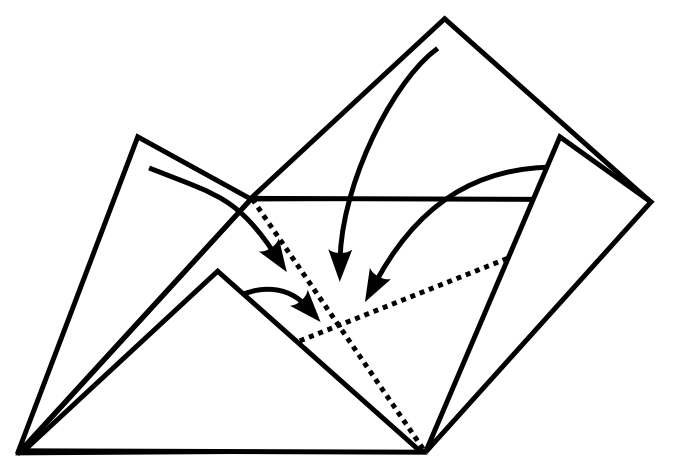
\includegraphics[width=2in]{fold}

\vskip -.9in {\gr One option is to just take \\repeated random samples.
\\
It is better to `fold' your data.}

\vskip 1cm
$\bullet$ Sample a random ordering of the data \\ { ~~(important to avoid order dependence)}

\vskip .1cm $\bullet$ Split the data into $K$ folds: { 1st 100/K\%, 2nd 100/K\%, etc}.

\vskip .1cm 
$\bullet$ Cycle through $K$ CV iterations with a single fold left-out.

\vskip .25cm
This guarantees each observation is left-out for validation, \\and lowers the sampling variance of CV model selection.

\vskip .25cm
Leave-one-out CV, with $K=n$, is nice but takes a long time.\\
$K=5$ to $10$ is fine in most applications.

\end{frame}


\begin{frame}
{CV Lasso}

The lasso path algorithm minimizes $-\frac{2}{n}\log\text{LHD}(\bs{\beta}) + \lambda_t \sum_j |\beta_j|$ over the sequence of penalty weights $\lambda_1 > \lambda_2 \ldots > \lambda_T$.

\vskip .25cm
This gives us a path of $T$ fitted coefficient vectors, 
$\nv \bs{\hat\beta}_1 \ldots \bs{\hat\beta}_T$,
each defining deviance for new data: $\nv -\log \text{p}(\bm{y}^{new}\mid\bm{X}^{new}\bs{\hat\beta}_t)$.

\vskip .5cm
Set a sequence of penalties $\lambda_1 \ldots \lambda_T$.  \\
Then, for each of $k=1\ldots K$ folds,
\begin{itemize}
\item Fit the path $\nv \bs{\hat\beta}^k_1 \ldots \bs{\hat\beta}^k_T$ on all data {\it except} fold $k$.
\item Get fitted deviance {\it on left-out data}: 
$\nv -\log \text{p}(\bm{y}^{k}\mid\bm{X}^{k}\bs{\hat\beta}_t)$.
\end{itemize}

This gives us $K$ draws of OOS deviance for each $\lambda_t$.

\vskip .5cm
Finally, use the results to choose the `best' $\theme \hat\lambda$, then re-fit the model to {\it all of the data} 
by minimizing $-\frac{2}{n}\log\text{LHD}(\bs{\beta}) 
+ {\theme \hat \lambda} \sum_j |\beta_j|$.

\end{frame}


\begin{frame}[fragile]
{CV Lasso}

{Both {\tt gamlr} and {\tt glmnet} have functions to wrap this all up.}

The syntax is the same; just preface with {\tt cv.}

\begin{semiverbatim}\nv
cv.spender <- cv.gamlr(xweb, log(yspend))
\end{semiverbatim}

Then, {\nv\tt coef(cv.spender)} gives you $\bs{\hat\beta}_t$ at the `best' $\lambda_t$
\begin{itemize}
\item {\tt select="min"} gives $\lambda_t$ with {\it min average OOS deviance}.
\item {\tt select="1se"} defines best as {\it biggest $\lambda_t$ with average OOS deviance no more than 1SD away from the minimum.}
\end{itemize}

\vskip .2cm
{\tt 1se} is default, and balances prediction against false discovery.  

{\tt min} is purely focused on predictive performance.

\end{frame}


\begin{frame}
{CV Lasso}

\vskip .25cm

Again, the routine is most easily understood visually.

\vskip -.25cm
\begin{center}
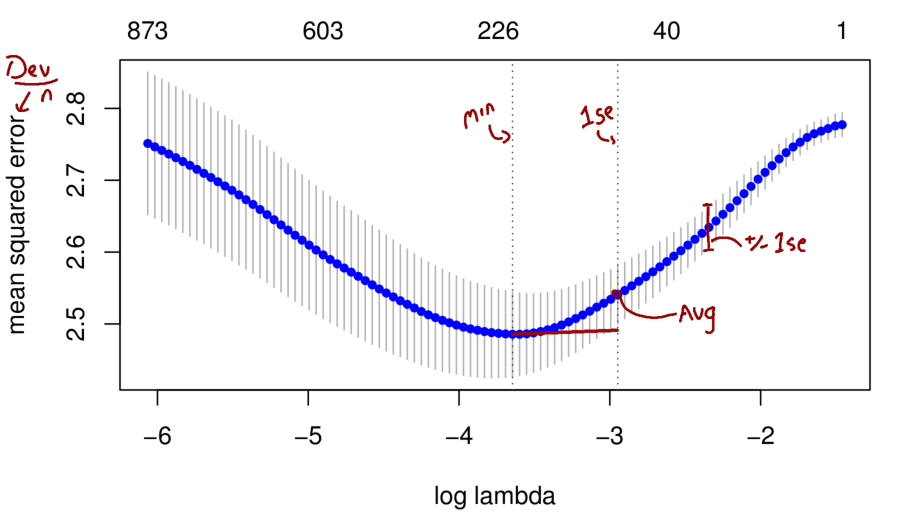
\includegraphics[width=\textwidth]{comscore_cvmarkedup}
\end{center}

\vskip -.25cm
Both selection rules are good; {\tt 1se} has extra bias for simplicity.
\end{frame}

\begin{frame}[fragile]
{\gr Alternatives to CV: \bk Information Criteria}

\vskip .25cm
{Many `Information Criteria' out there: AICc, AIC, BIC, ...}

These approximate distance between a model and `the truth'.

You can apply them by choosing the model with minimum IC.

\sk
Most common is Akaike's {\theme AIC = Deviance + $2df$.}

\vskip .2cm
$df$ = `degrees of freedom' used in your model fit.

For lasso and MLE, this is just the $\#$ of nonzero $\hat\beta_j$.

\end{frame}

\begin{frame}
{AIC overfits in high dimensions}

The AIC is atually estimating OOS deviance: 
what your deviance would be on another {\it independent} sample of size $n$.

\vskip .5cm
IS deviance is too small, since the model is tuned to this data.  \\Some deep theory shows that IS - OOS deviance $\approx 2df$.
\vskip .1cm

\hskip 2in $\Rightarrow \text{AIC} \approx$ OOS deviance.

\sk
Its common to claim this approx (i.e., AIC) is good for `big $n$'.

{\theme Actually, its only good for big $n/df$. } 

\sk
In Big Data, $df$ (\# parameters) can be huge.  Often $df\approx n$.

In this case the AIC will be a bad approximation: it overfits!

\end{frame}

\begin{frame}
{AIC corrected: \nv AICc}

AIC approximates OOS deviance, but does a bad job for big $df$.
 
\sk
In linear regression an improved approx to OOS deviance is
\[
\theme \text{AICc} { ~\gr = \text{Deviance} + 2df\ds{E}\left[\frac{\sigma^2}{\hat \sigma^2}\right]} = \text{Deviance} + 2df\frac{n}{n-df-1}
\]
This is the corrected AIC, or AICc.  

\vskip .05cm
{It also works nicely in logistic regression, or for any {\tt glm}.}

\vskip .5cm
Notice that for big $n/df$, AICc $\approx$ AIC. So {\it always} use AICc.

\end{frame}

\begin{frame}[fragile]
{gamlr uses AICc}

\vskip .25cm

{It's marked on the path plot}

\vskip .25cm
\hskip .5in 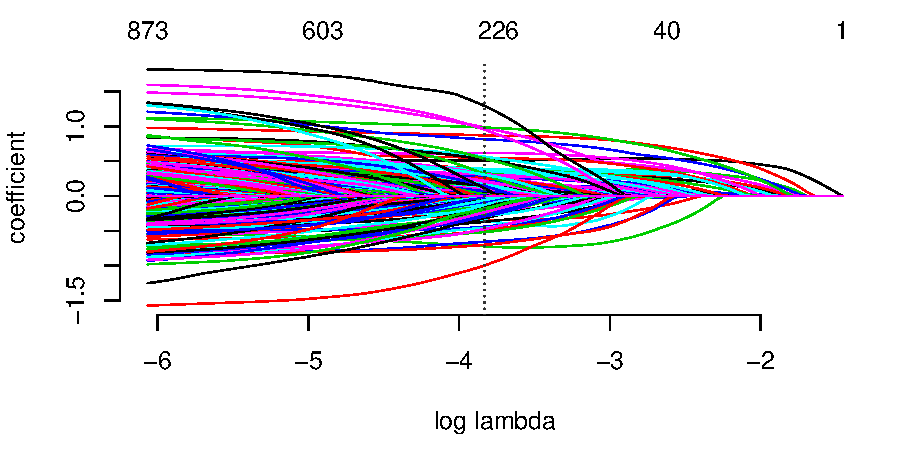
\includegraphics[width=.8\textwidth]{comscore_pathaicc}

\vskip .1cm
And it is the default for {\tt coef.gamlr}

\begin{semiverbatim}\nv\small
B <- coef(spender)[-1,] 
B[c(which.min(B),which.max(B))]\bk
    cursormania.com shopyourbargain.com 
          -0.998143            1.294246 
\end{semiverbatim}

\end{frame}

\begin{frame}
{{\gr Another option: } Bayes IC}

The BIC is  {\nv Deviance + $\log(n)\times df$}.

\vskip .05cm
This {\it looks} just like AIC, but comes from a very different place.

\vskip .25cm
$BIC \approx -\log \mr{p}(M_b|\mr{data})$, the `probability that model $b$ is true'.
\[
\mr{p}(M_b|\mr{data}) = \frac{\mr{p}(\mr{data}, M_b)}{\mr{p(data)}} 
\propto \gr\underbrace{\bk\mr{p}(\mr{data}|M_b)}_\text{LHD}
\underbrace{\bk\mr{p}(M_b)}_{\text{prior}}
\]
The `prior' is your probability that a model is true {\it before} you saw any data. {\gr BIC uses a `unit-info' prior: 
$\mr{N}\!\left[\bs{\hat\beta}, \frac{2}{n}\mr{var}(\bs{\hat\beta})^{-1}\right]$}

\vskip .25cm
AIC[c] tries to approx OOS deviance.\\
 BIC is trying to get at the `truth'.


\end{frame}

\begin{frame}
{IC and CV on the Comscore Data}

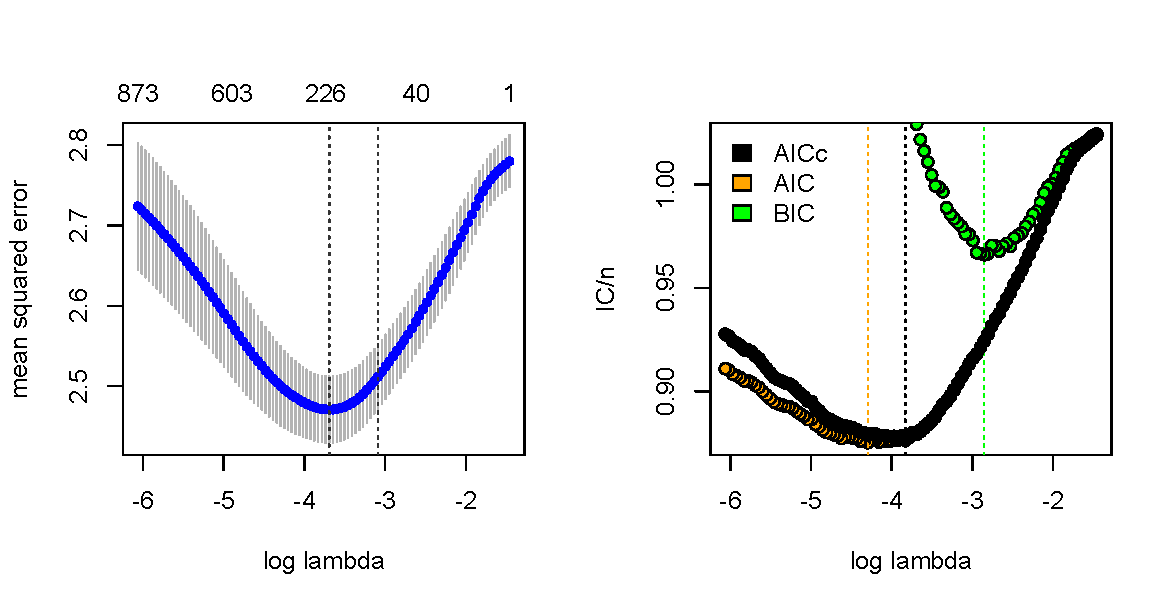
\includegraphics[width=\textwidth]{comscore_icvcv}

\sk
The take home message: AICc curve looks like CV curve.

 \vskip .25cm
In practice, BIC works more like the 1se CV rule.  \\
But with big $n$ it chooses too simple models (it underfits).

\end{frame}


\begin{frame}
{IC and CV on the Comscore Data}

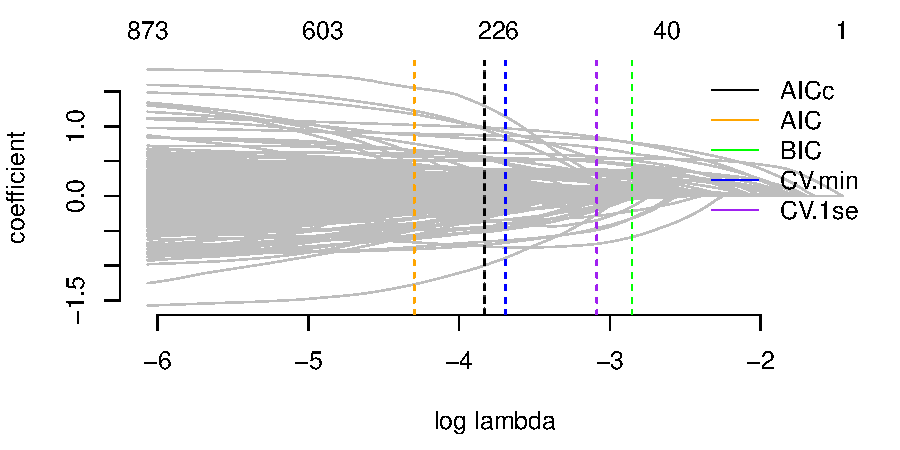
\includegraphics[width=\textwidth]{comscore_pathallic}

\vskip .2cm
With all of these selection rules, you get a range of answers.

If you have time, do CV.  But AICc is fast and stable.

If you are worried about false discovery, tend towards BIC/1se.

\end{frame}




\begin{frame}


{\bf Decision Trees}

\vskip .5cm
Trees are great: nonlinearity, deep interactions, heteroskedasticity.

\begin{center}
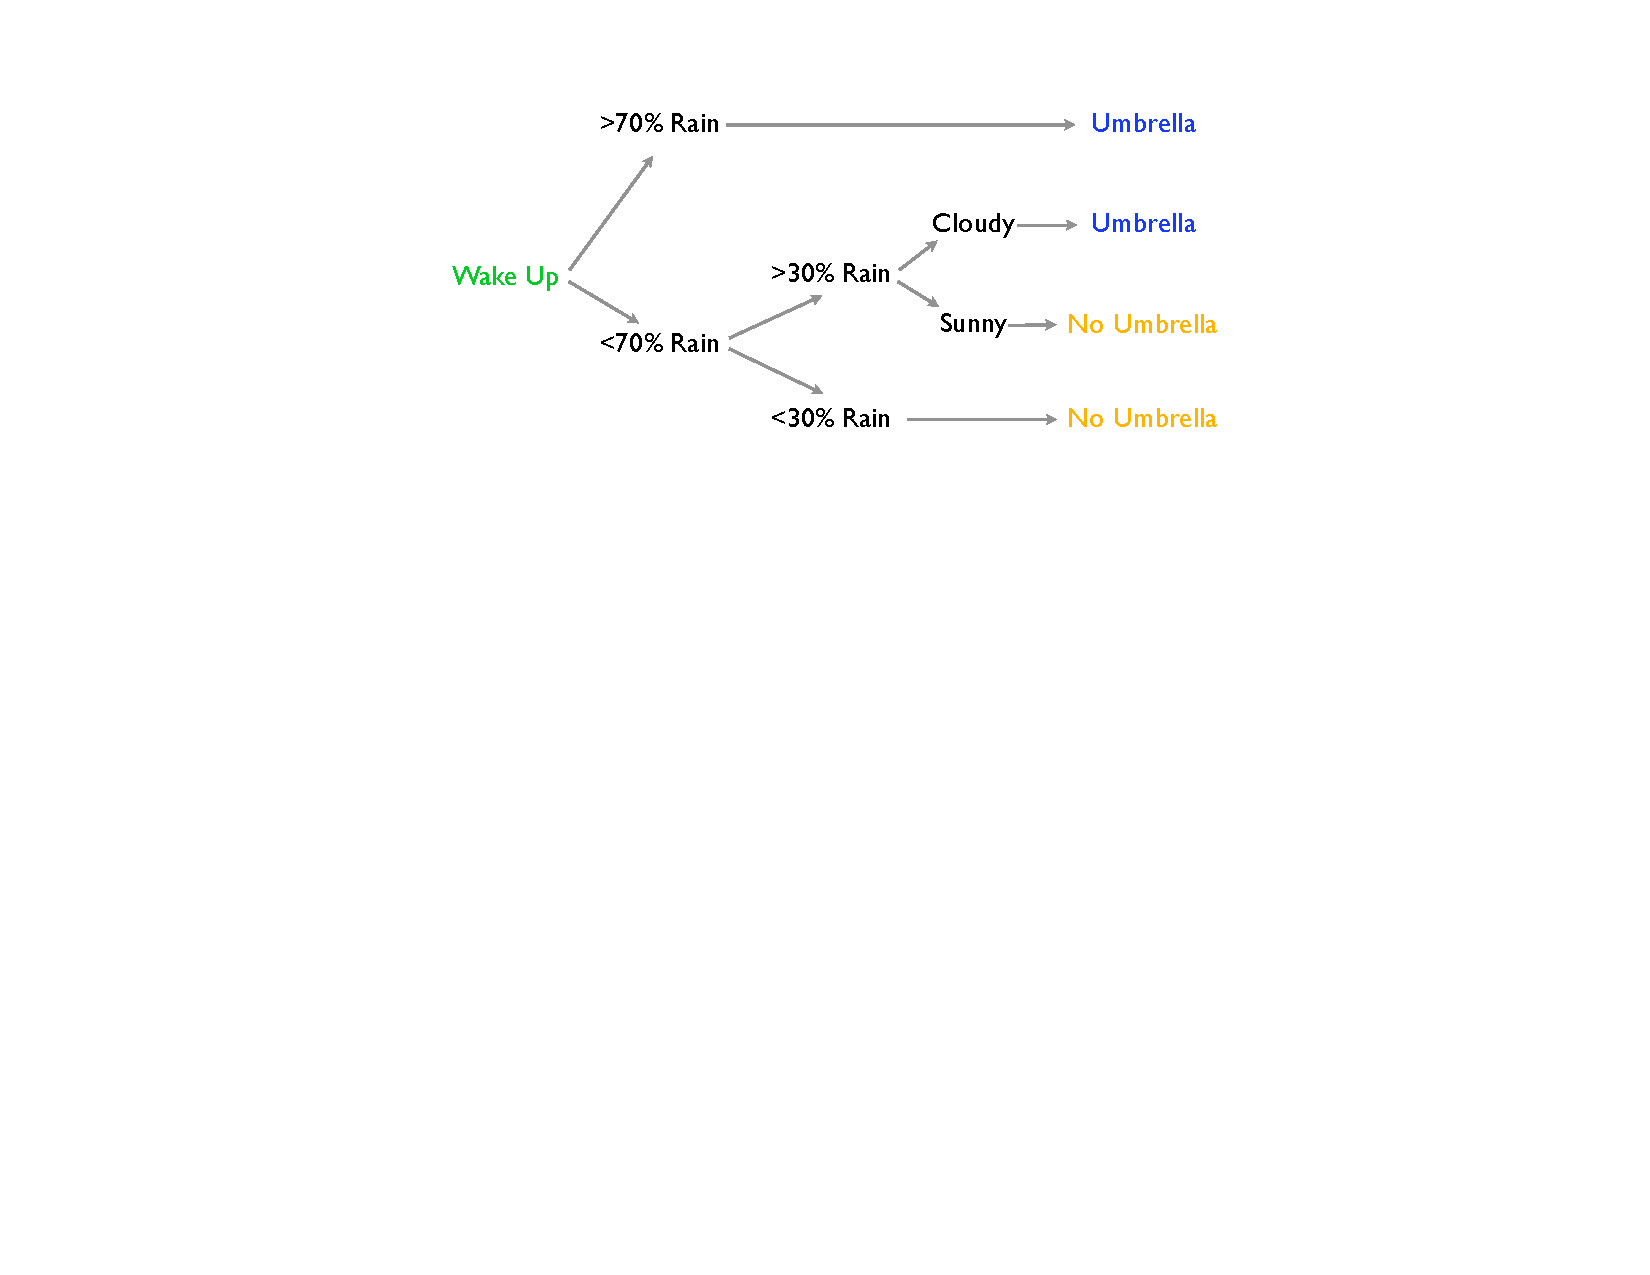
\includegraphics[width=4in]{../graphs/umbrella}
\end{center}

The `optimal' decision tree is a statistic we care about {\gr (s.w.c.a)}.


\end{frame}


\begin{frame}


{\bf {\theme CART:} greedy growing with optimal splits}

\vskip .5cm
Given node $\{\bm{x}_i,y_i\}_{i=1}^n$ and DGP weights $\bs{\theta}$,
find $x$ to minimize 
\begin{align*}
|\bs{\theta}|\sigma^2(x, \bs{\theta} ) &= \sum_{k \in \mathrm{left}(x)} \theta_k (y_k - \mu_{\mathrm{left}(x)})^2 \\&+ \sum_{k \in \mathrm{right}(x)} \theta_k (y_k - \mu_{\mathrm{right}(x)})^2
\end{align*}
for a regression tree.  Classification impurity can be Gini, etc.


\end{frame}























\begin{frame}


{\bf  Trees are awesome}

\vskip .25cm 
They automatically learn non-linear response functions
\\ and will discover interactions between variables.

\vskip .25cm
Example: Motorcycle Crash Test Dummy Data

\sg
$x$ is time from impact, $y$ is acceleration on the helmet.

\vspace{-1cm}
\begin{adjustwidth}{-.3in}{}
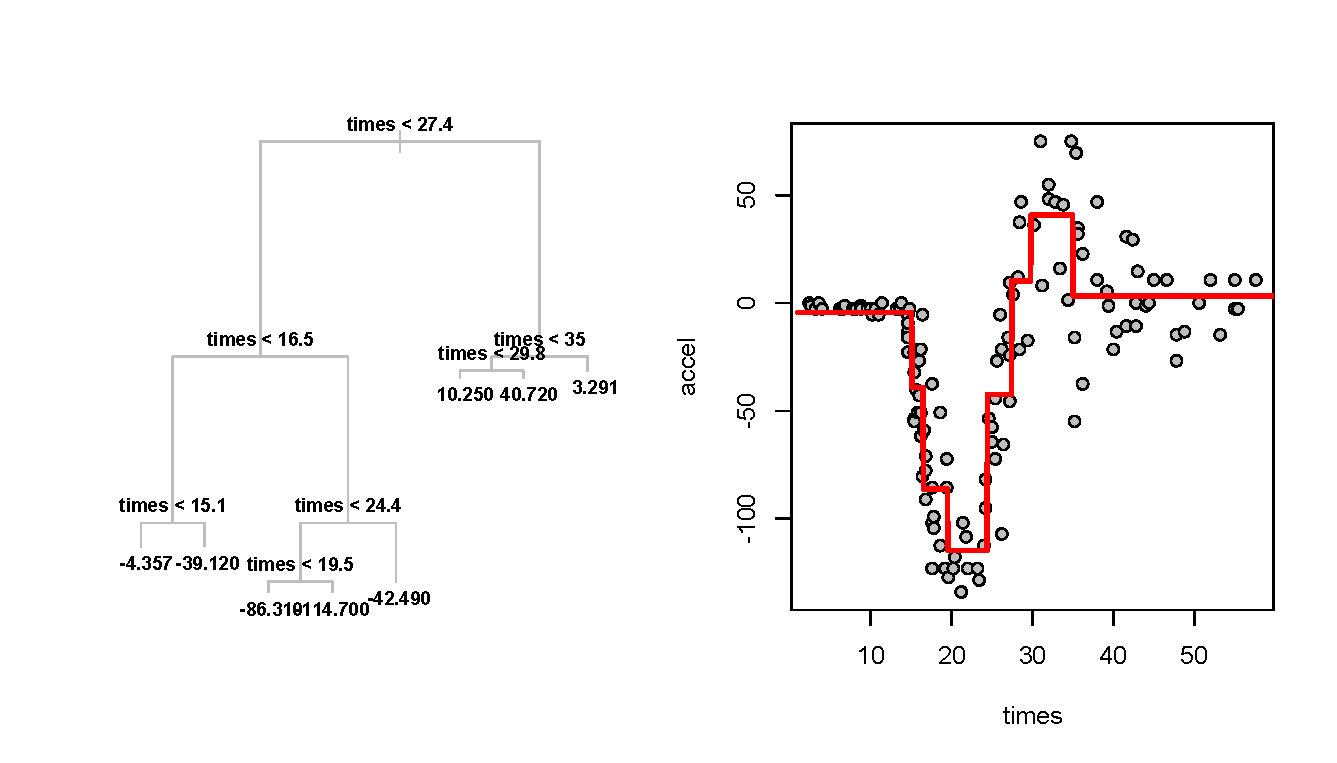
\includegraphics[width=4.6in]{../graphs/MCtree}
\end{adjustwidth}

\vskip -.75cm
\end{frame}


\begin{frame}

{Unfortunately, deep tree structure is so unstable that optimal depth is not easily chosen via cross validation}

\begin{itemize}
\item tree  predictions are non-smooth wrt the tuning parameter (tree depth).
\item Breiman 2001: \rd Cross-validation fails for such tuning
\end{itemize}

\end{frame}

\begin{frame}
\vskip .5cm \bk
Instead, we can average over a {\nv bootstrapped} sample of trees:  

\begin{itemize}
\item repeatedly re-sample the data, {\nv with-replacement}, \\to get a `jittered' dataset of $n$ observations.
\item for each resample, {\nv fit a CART tree}.
\item when you want to predict $y$ for some $\bm{x}$, \\take the {\nv average} prediction from this forest of trees.
\end{itemize}
Real structure that persists across datasets shows up in the average.  Noisy useless signals will average out to have no effect. 

\sk
{\bf \theme \hfill This is a Random Forest}
\end{frame}

\begin{frame}

{\bf \theme Random Forests}

\bk
\vskip .25cm
$\bullet$ Sample $B$ subsets of the data {\tt +} variables: \\ ~~~e.g., 
observations $1,5,20,...$ and inputs $2,10,17,...$

\vskip .2cm
$\bullet$ Fit a tree to each subset, to get $B$ fitted trees is $\mc{T}_b$.

\vskip .2cm
$\bullet$
Average prediction across trees:

\vskip .1cm
 ~~~~ -  for regression average $\ds{E}[y|\bm{x}] = \frac{1}{B}\sum_{b=1}^B \mc{T}_b(\bm{x})$.

 \vskip .1cm
 ~~~~ -  for classification let $\{\mc{T}_b(\bm{x})\}_{b=1}^B$ vote on $\hat y$.

\vskip .25cm
{\gr The observation resample is usually {\it with-replacement}, so that this is taking the {\it average of bootstrapped trees} (i.e., `bagging')}

\end{frame}

\begin{frame}

{\bf Understanding \theme Random Forests}

\sk Recall how CART is used in practice.
\begin{itemize}
\item Split to lower deviance until leaves hit minimum size.
\item Create a set of candidate trees by pruning back from this.
\item Choose the best among those trees by cross validation.
\end{itemize}

\sk {\nv Random Forests avoid the need for CV.}

\vskip .1cm Each tree `$b$' is not overly complicated 
because \\you only work with a  limited set of variables.

\vskip .1cm Your predictions are not `optimized to noise' 
because \\they are averages of trees fit to many different subsets.

\sk
RFs are a great go-to model for nonparametric prediction.
%\\{\gr As with all trees, they're not great in high ($>100$) dimension.}

\end{frame}


\begin{frame}

{\bf\theme Deeper: \bk Distribution-free Bayesian nonparametrics}

\vskip .5cm
{Find some {\it statistic of the DGP} that you care about:}
\vskip .1cm
\begin{itemize}
\item derive from first principles, e.g. moment conditions
\item {\it an algorithm} that we know works, e.g. CART
\item think about geometric projections, e.g. OLS
\end{itemize}
\vskip .1cm
Call this statistic $\bs{\theta}(g)$ where $g(\bm{z})$ is the DGP (e.g., for $\bm{z} = [\bm{x},y]$).

\vskip .5cm
Then you write down a flexible  model for the DGP $g$, and study properties of the posterior on $\bs{\theta}(g)$ induced by the posterior over $g$.

\end{frame}

\begin{frame}

{\bf A flexible model for the DGP}

\vskip .5cm
Say $\bm{z} = [\bm{x},y]$ is a single {\it independent} data point.

\vskip .25cm Each data point assumes one of a {\it finite} number of possible values, $[\bs{\zeta}_1 \ldots \bs{\zeta}_L]$, with probabilities proportional to $[\bs{\theta}_1 \ldots \bs{\theta}_L]$.
\begin{equation*}
g(\bm{z}) = \frac{1}{|\bs{\theta}|}\sum_{l=1}^L \theta_l \ds{1}_{[\bm{z} =
\bs{\zeta}_l]}\end{equation*}

We complete specification with a conjugate prior on the weights:
\[\frac{\bs{\theta}}{|\bs{\theta}|} \sim \mr{Dir}(a) \propto \frac{1}{|\bs{\theta}|^{L(a-1)}}\prod_l \theta_l^{a-1}~~\text{where}~~a,\theta_l >0.
\]
%The support is treated as fixed.

%\vskip .25cm
This is the Dirichlet-multinomial sampling model {\gr (Ferguson 1973)}.  

\end{frame}

\begin{frame}

Now you've observed some data, say $\bm{Z} = \{\bm{z}_1 \ldots \bm{z}_n\}$.\\
{\gr (say every $\bm{z}_i = [\bm{x}_i,y_i]$ is unique)}.

\vskip .25cm
The posterior over weights has $\theta_l \stackrel{ind}{\sim} \mr{Exp}\left(a+\ds{1}_{[\bs{\zeta}_l \in \bm{Z}]}\right)$. 

\vskip .5cm
{\bf A convenient limiting case}

\vskip .25cm
$a \to 0$ leads to $\mr{p}(\theta_l = 0) = 1$ for $\bs{\zeta}_l \notin \bm{Z}$.

\vskip .2cm
In this case, we can focus on only the {\it observed support} and write the posterior for our DGP
\[
g(\bm{z}) = \tfrac{1}{|\bs{\theta}|}
\sum_{i=1}^n \theta_i \ds{1}{[\bm{z} =
\bm{z}_i]},~~~\theta_i \stackrel{iid}{\sim} \mr{Exp}(1).
\]

\hfill
{This is just the Bayesian bootstrap. \gr (Rubin 1981)}

\end{frame}


\begin{frame}[fragile]

{\bf \theme Bayesian Forests: \bk a posterior for CART trees}

\vskip .25cm
For $b=1 \dots B$: \\
   ~~~~~~~~~~$\bullet$ draw $\boldsymbol{\theta}^b \stackrel{iid}{\sim} \mathrm{Exp}(\mathbf{1})$
   \\
   ~~~~~~~~~~$\bullet$ run weighted-sample CART to get $\mathcal{T}_b = \mathcal{T}(\boldsymbol{\theta}^b)$
 
\vskip .5cm\small 
~~~~~~~~~~~~~~~~~~~~~{\it one tree~~~~~~~~~~~~~~~~~~~~~~~~~~~~~~~~~~posterior mean}\\

\includegraphics[height=1.75in]{../graphs/MCtreedraw}   
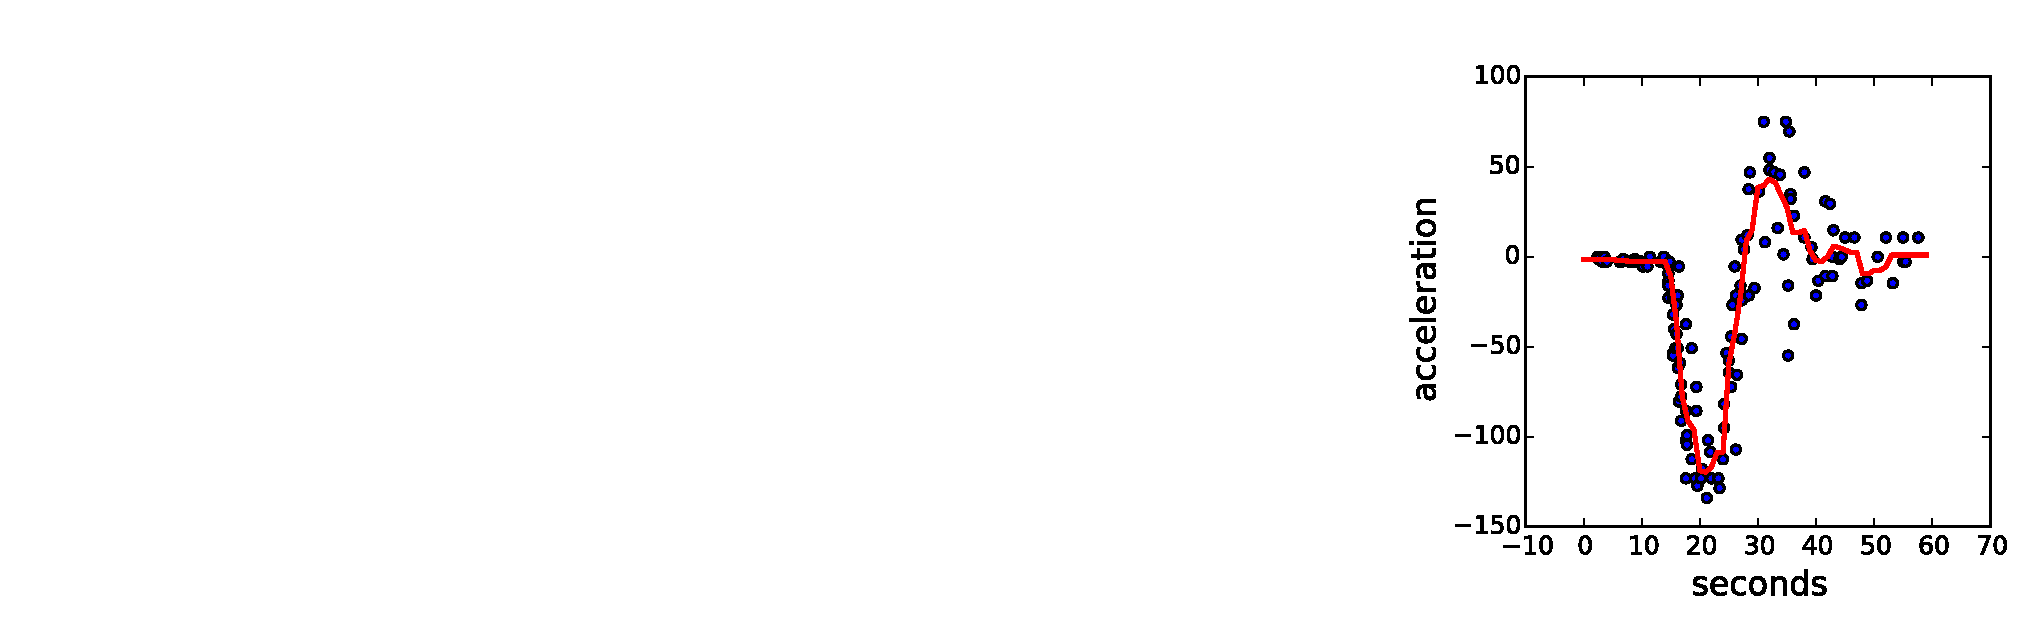
\includegraphics[height=1.75in]{../graphs/MCbforest}   

\vskip .25cm{
Random Forest $\approx$ Bayesian forest $\approx$ posterior over CART fits.}

\vskip -.5cm

\end{frame}

\begin{frame}[fragile]

{\bf Random Forests in R}

\vskip .25cm

R has the {\tt randomForest} package, \\which
works essentially the same as {\tt tree}

\vskip .1cm{\small \nv
~~~~\verb|spamrf <- randomForest(spam ~ ., data=xemail)|
}
\vskip .25cm 
{\gr For big datasets, use ${\tt x = x,  ~y=y}$ like in {\tt gamlr}}.


\sk
{\nv Unfortunately, you lose
the interpretability of a single tree.}

However, if you set {\tt importance=TRUE}, {\tt Random Forest}
will evaluate each $\mc{T}_b$'s performance on the {\it left-out sample}
(recall each tree is fit on a sub-sample).  This yields nice OOS stats.

\vskip .25cm
They can be slow (due to many tree fits) but\\
they can also be fit in parallel or on distributed data...

\end{frame}



\begin{frame}


\begin{center}

\includegraphics[width=.75\textwidth]{../graphs/MCtreedraw}
\end{center}

\vskip -.25cm
Fitting CART to sampled-with-replacement data is equivalent to randomly {\nv weighting} your observations in the deviance calculations. 

\hfill {\gr (size proportional to weight in this picture)}.

\end{frame}

\begin{frame}

{\bf \theme Random Trees \bk for the Motorcycle Data}


\vspace{-1cm}
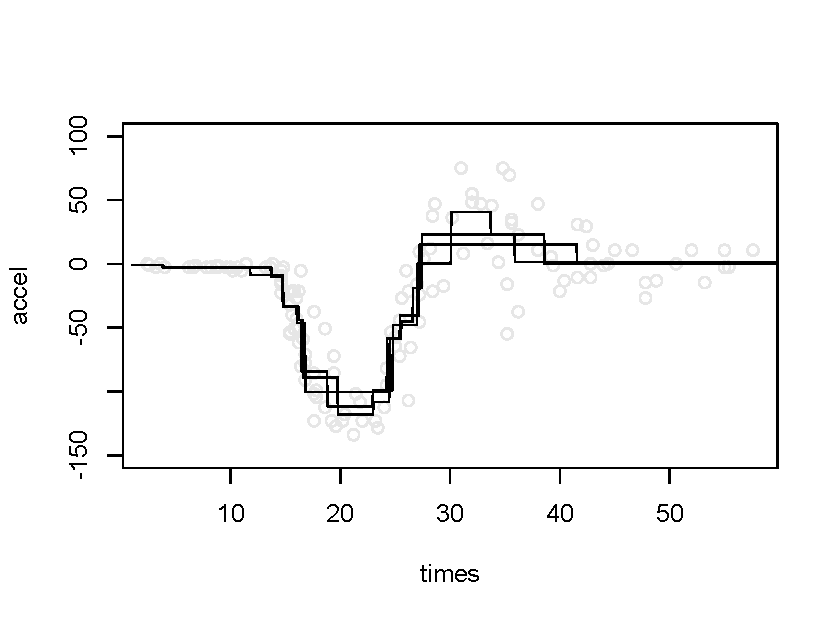
\includegraphics[width=4.25in]{../graphs/MCparticles}

\vskip -.25cm\sg
If you fit to random subsets of the data, \\\nv \hfill you get a slightly different
tree each time.
\vskip -.25cm
\end{frame}


\begin{frame}

{\bf  Model Averaging with \theme Random Forests}

\vskip .25cm
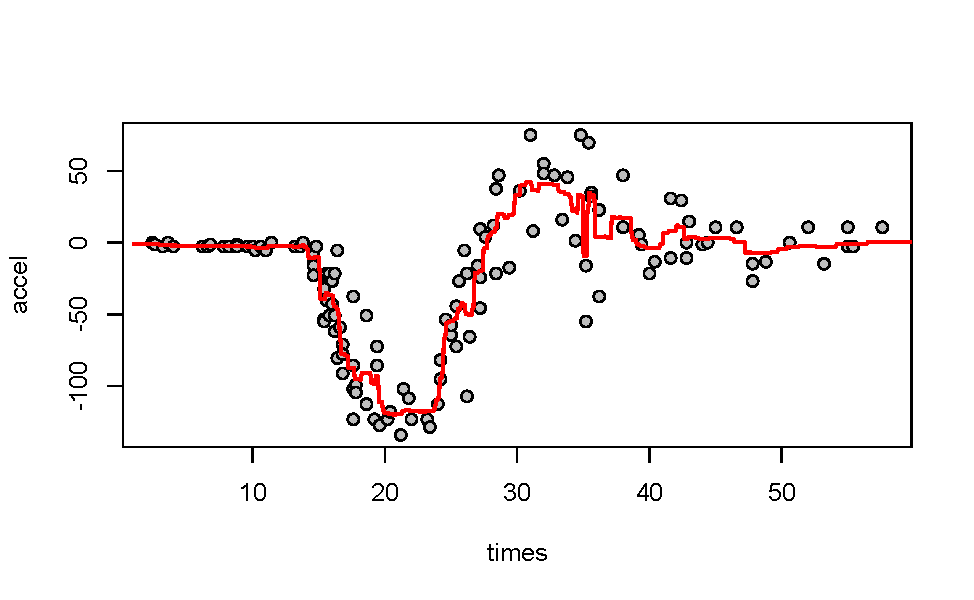
\includegraphics[width=4.35in]{../graphs/MCrf}

\vskip .2cm\sg
Averaging many trees yields a single
response surface. \\ \gr \it Still looks like a bit of overfit to me, which remains a
danger.

\vskip -.2cm

\end{frame}



\begin{frame}

{\bf A larger example: \theme California Housing Data}

\sk
Median home values in census tracts, along with
\begin{itemize}
\item Latitude and Longitude of tract centers.
\item Population totals and median income.
\item Average room/bedroom numbers, home age.
\end{itemize}
The goal is to predict {\nv log(MedVal)} for census tracts.


\sk
Difficult regression: \sg Covariate effects change with location.
\\\gr ~~~~~~~~~~~~~~~~~~~~~~~~~How they change is probably not linear.
\end{frame}


\begin{frame}

{\bf \theme CART Dendrogram for  CA housing}


\vspace{-1cm}
\begin{adjustwidth}{-.5in}{}
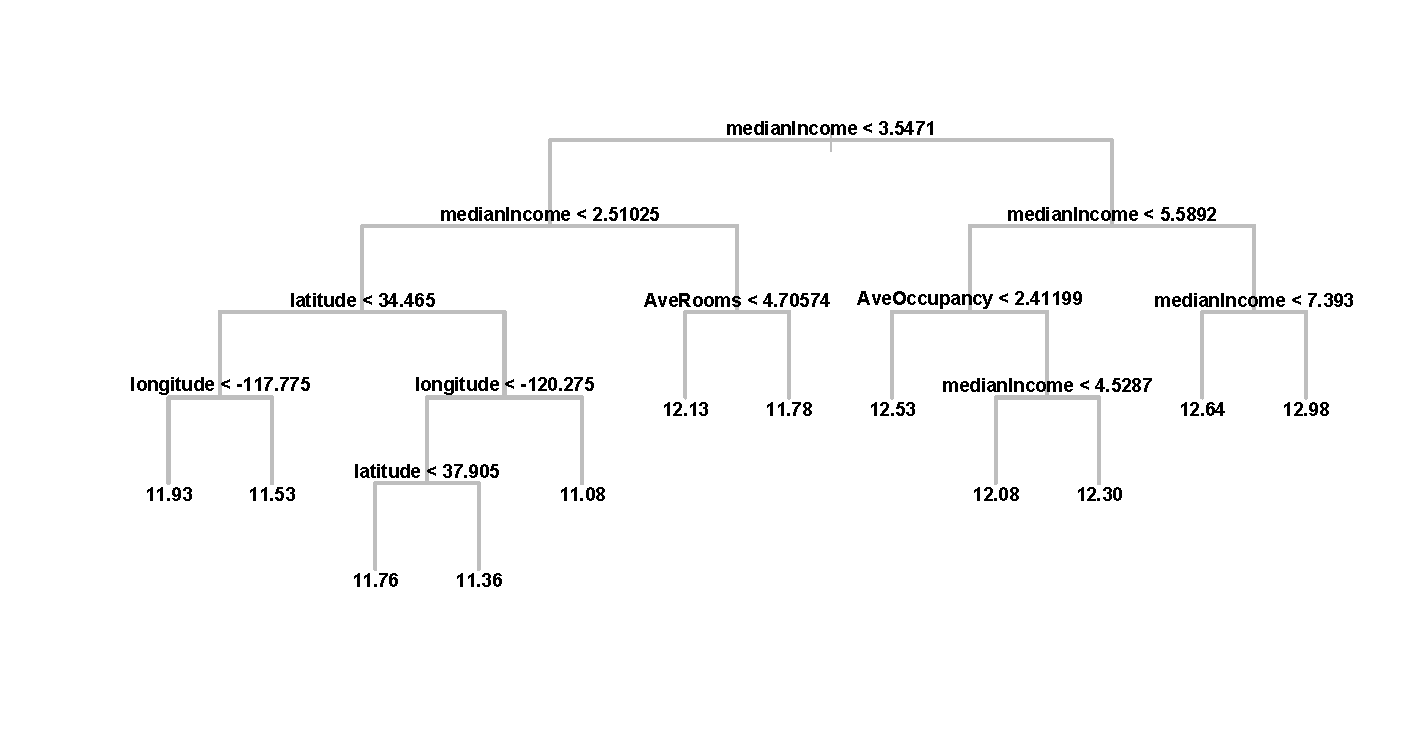
\includegraphics[width=5in]{../graphs/CAHtree}
\end{adjustwidth}

\vspace{-1cm}
\sg Income is dominant, with location important for low income.\\
\gr  Cross Validation favors the most complicated tree: 12 leaves.
\end{frame}


\begin{frame}

{\bf \theme LASSO \gr fit for CA housing data}

\vskip .2cm
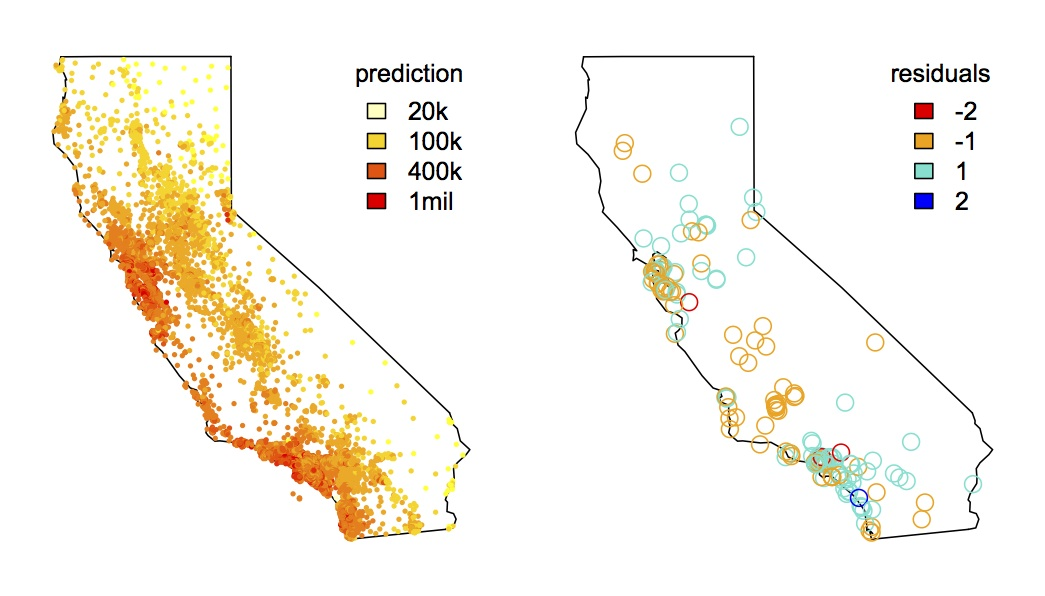
\includegraphics[width=4.25in]{../graphs/CAHlinpredSMALL}

\gr
Looks like over-estimates in the Bay, under-estimates in OC.
\end{frame}


\begin{frame}

{\bf \theme CART \gr fit for CA housing data}

\vskip .2cm
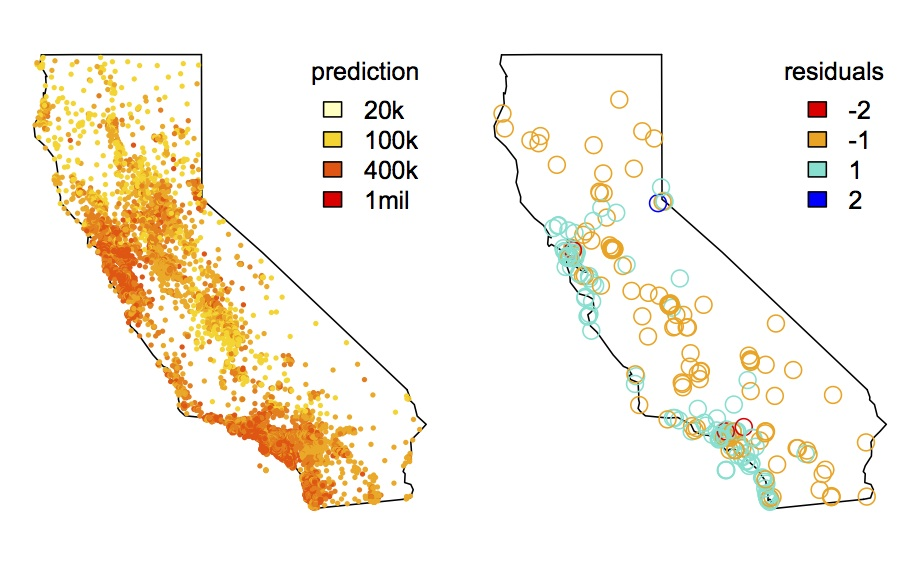
\includegraphics[width=4.25in]{../graphs/CAHtreepredSMALL}

\gr
Under-estimating the coast, over-estimating the central valley?
\end{frame}

\begin{frame}[fragile]

{\bf \theme randomForest \gr fit for CA housing data}

\vskip .2cm
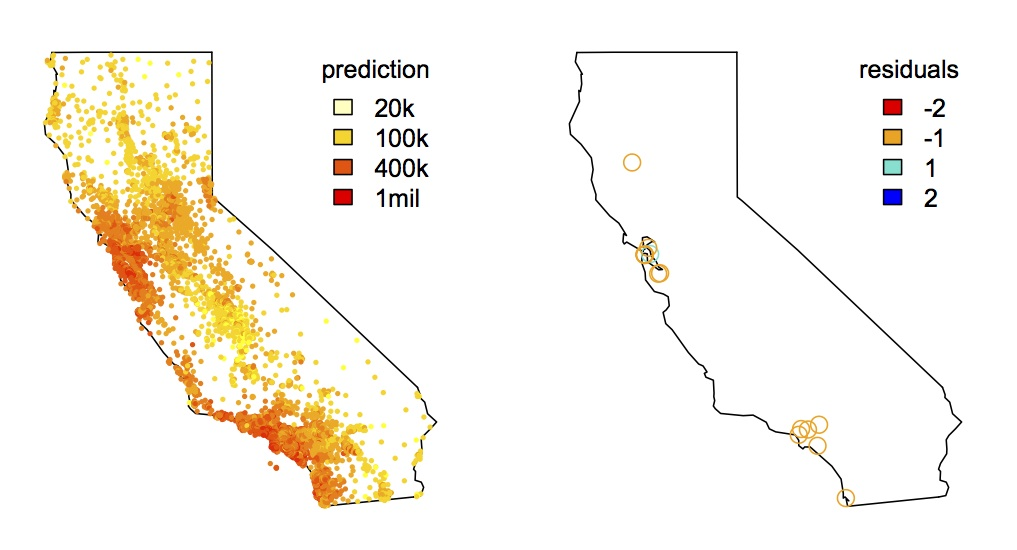
\includegraphics[width=4.25in]{../graphs/CAHrfpredSMALL}

No big residuals!  (although still missing the LA and SF effects)  \\\gr Overfit?  From out-of-sample prediction it
appears not.
\vskip -.15cm
\end{frame}

\begin{frame}

{\bf \theme CA housing: \bk out-of-sample prediction}

\vskip .5cm
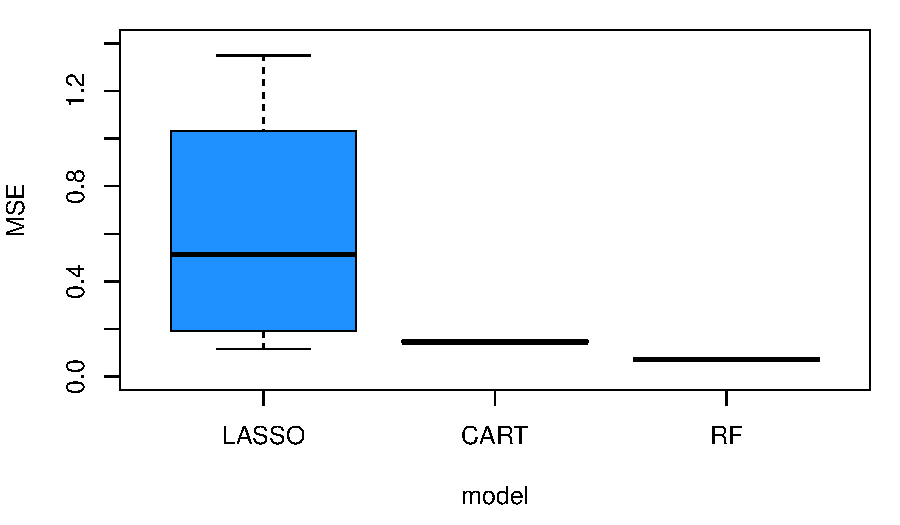
\includegraphics[width=4.25in]{../graphs/calhomesMSE}

Trees outperform LASSO:  ~gain from  nonlinear interaction.\\
RF is better still than CART: ~benefits of model averaging. 
\vskip -.25cm
\end{frame}



\begin{frame}
{Aside: trunks are stable (Taddy+ icml 2015)}
\begin{columns}

\begin{column}{2.15in}
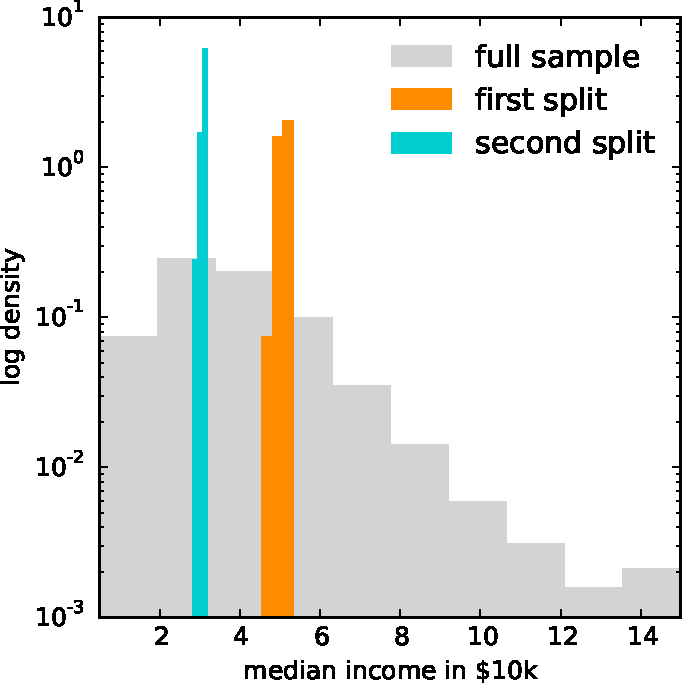
\includegraphics[width=2.5in]{../graphs/ca_splits}
\end{column}

\begin{column}{2in}
\begin{itemize}
\item sample tree occurs 62\% \\of the time.  
\vskip .5cm
\item 90\% of  trees split on income twice, \\and then latitude. 

\vskip .5cm
\item 100\% of trees have 1st 2 splits on median income.  
\end{itemize}
\end{column}

\end{columns}


\vskip 1cm
~~~~Empirically and theoretically: trees are stable, at the trunk.
\vskip -1cm

\end{frame}

\begin{frame}

{\bf Random Forest {\theme bottlenecks}}

\vskip .5cm
RFs (or BFs) are awesome, but when the data are too big to fit in memory or on a single machine they get extremely expensive.\\ {\gr \small (e.g., Google PLANET, Panda 2009)}.

\vskip .5cm
A common solution is a `sub-sampling forest': instead of drawing with-replacement, or re-weighting, draw $m \ll n$ sub-samples.

\vskip .5cm
This defeats the whole purpose of trees: these are rules that are designed to grow in complexity with the amount of data available. {\gr(that's why we bother storing so much data!)}

\vskip .5cm If you starve the individual trees of data you lose.

\end{frame}

% \begin{frame}
% \begin{adjustwidth}{-.5in}{}
% \vskip -.6in
% 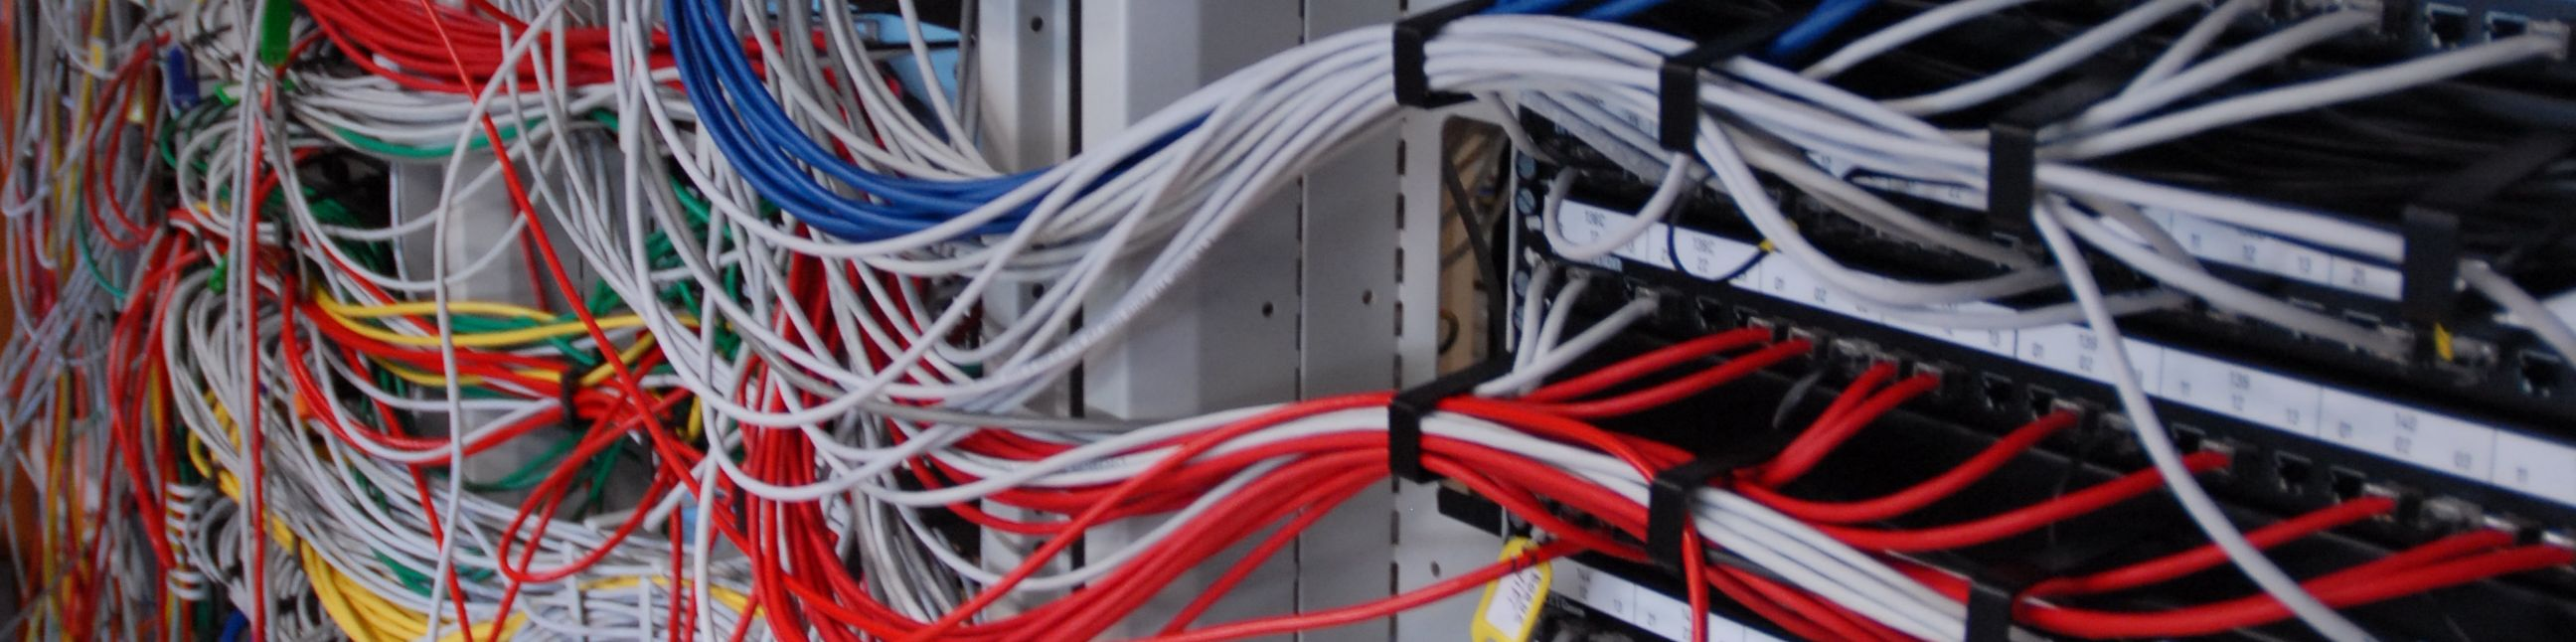
\includegraphics[width=6in]{../graphs/broadband}
% \end{adjustwidth}

% \vskip .6cm

% { \bf Data Distribution and Big Data}

% \vskip .5cm
% {\nv Distributed}: independent computations on many datasets.\\

% \vskip .1cm
% For truly {\nv Big Data} we need distributed algorithms.

% \vskip .5cm
% The trick is to find strategies for distribution so that local-machine calculations are as relevant as possible to the global inference question:
% only data that needs to be together is together.

% \end{frame}



\begin{frame}

{\bf Empirical Bayesian Forests ({\theme EBF})}

\vskip .5cm
RFs are expensive.  Sub-sampling hurts bad.

\vskip .25cm
{Instead:}
\begin{itemize}
\item fit a single tree to a shallow {\nv trunk}.  
\item Map data to each {\nv branch}.  
\item Fit a full  forest on the smaller branch datasets.
\end{itemize}

\vskip .25cm
Since the trunks are all similar for each tree in a full forest,
our EBF looks nearly the same at a fraction of computational cost.

\vskip .5cm
It's an updated version of classical {\theme Empirical Bayes}: \\ ~~~use plug-in estimates at high levels in a hierarchical model, \\~~~focus effort at full Bayesian learning for the the hard bits.


\end{frame}

\begin{frame}

{\bf OOS predictive performance on California Housing}




\begin{center}
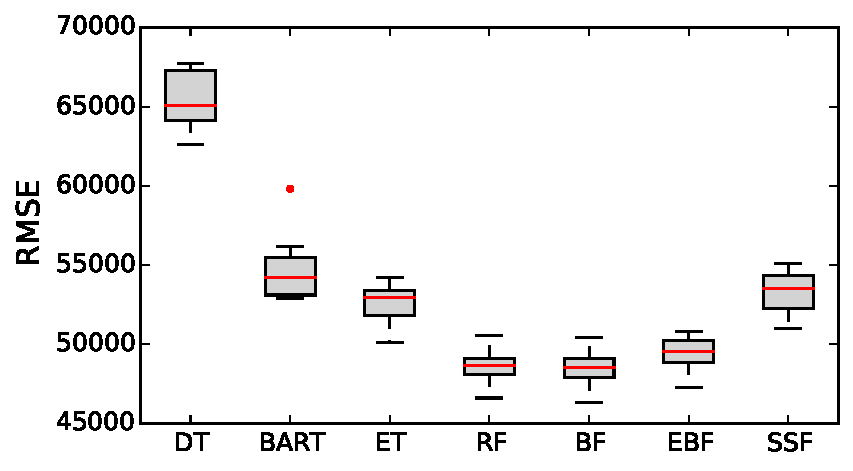
\includegraphics[width=.85\textwidth]{../graphs/ca_rmse}
\end{center}

Here EBF and BF give nearly the same results.  {\it SSF does not.}

\vskip .25cm
EBFs crunch more data faster without hurting performance.


\end{frame}



\begin{frame}

{\bf Roundup on  {\theme Tree-based learning}}

\vskip .25cm

We've seen two techniques for building tree models.
\begin{itemize}
\item {\nv CART:} recursive partitions, pruned back by CV.
\item {\nv randomForest:} average many simple CART trees.
\end{itemize}

\vskip .25cm
There are many other tree-based algorithms.
\begin{itemize}
\item {\nv Boosted Trees:} repeatedly fit simple trees to residuals.\\
{\gr Fast, but it is tough to avoid over-fit (requires full CV).}
\item {\nv Bayes Additive Regression Trees:} mix many simple trees.\\
{\gr Robust prediction, but suffers with non-constant variance.}
\end{itemize}

\vskip .25cm
{\bk Trees are poor in high dimension,  but fitting them to
low dimension factors (principle components) is a good option.}

\vskip -.2cm

\end{frame}

\begin{frame}

{\bf Roundup on  {\theme  Nonlinear Regression} and  {\theme  Classification}}


\vskip .25cm
Many other {\it semiparametric learning} algorithms
\begin{itemize}
\item Neural Networks (and deep learning):\\{\gr many recursive logistic
  regressions.}
\item Support Vector Machines: \\{\gr Project to HD, then
  classify.}
\item Gaussian Processes, splines, wavelets, etc: \\{\gr Use sums of curvy functions in regression.}
\end{itemize}

\vskip .25cm
Some of these are great, but all take a ton of tuning.

{\gr Lots of work on automating this tuning for deep nets}

\vskip .25cm
{{\theme For now,} nothing's better out-of-the-box  in low-D than forests.}

\nv
But: \bk a lasso will tend to work better in high-D
\end{frame}



\end{document}